\section{Introduction}\label{sec:intro}

%
% The first version of introduction
%

%The appearance of search engines has largely changed people's way
%of using information in the age of information explosion.
%The rise of commercial search engines, such as Google, Bing or Yahoo,
%makes it easier and easier for people to find needed information.
%Every time we want to search about some particular information, we
%can simply type our \textit{needs} in the form of \textit{query} into
%a search engine. Over the years, many powerful features have been
%applied to search engines to improve users experiences.
%
%However, most of current commercial search engines are naturally
%keyword-based ones, which is not powerful enough in some certain
%scenarios. Take for an example, if a Vietnamese student wants to know about a
%hurricane that hit one of the states in US some time ago, but
%by chance he forgets the name of the state. For some specific name or entity
%that is not clearly remembered, our mind works by first trying to
%grasp an \textit{abstraction} of that specific \textit{instance}, which
%in this case the \textit{concept} of a ``state'' and a ``hurricane''.
%But, what will happen when the user put the query
%like ``hurricanes in states'' is that, with high certainty, the
%results will not be exactly relevant to the user's need. The results
%may contain some web pages  with a list of hurricanes, which are not
%the \textit{exact} thing or name that the user wanted, as shown in
%Fig. \ref{fig:exampleGoogle}.
%
%\textit{Here I can say something big about the project} In this work, we focus on solving this specific problem, so that search engines
%can give a more flexible user experience. In particular, given a query with vague
%terms (\textit{concept}),we are trying to replace the ambiguous terms with more
%specific ones and suggest users to use the returned queries to search for a better
%result. For the example stated above, our system is able to return ``hurricane katrina
%in florida'' or ``hurricane hugo in south carolina''. To achieve that, we come up with
%some algorithms and  include some essential tools, such as a probabilistic knowledge
%base (Probase \cite{wu2012probase}) and Stanford Parser \cite{klein2003accurate}.

%
% The second version of introduction
%

The quality of search results largely depend on the specificity
of the keywords they put in search engine, for modern search engine
are mostly keyword-based. When user queries do not general good results,
search engine may suggest a list of alternate queries for the user to
select and re-submit.

Traditionally, the function of query suggestion is implemented by
keyword-based methods and partially depends on the information from
search log \cite{baeza2005query,cao2008context,dupret2005recommending,zhang2006mining}, which includes click-through data, session data, etc.
%\KZ{What about these works:\cite{FonsecaGPRZ05,MeijBHHR09,BhatiaMM11}?}
With the rapid development of Internet, researchers are increasingly
interested in semantic view of the web and do a lot of work on semantic
relation extraction from search log \cite{baeza2007extracting} and
concept search \cite{giunchiglia2008concept,wang2012concept}.
There are also other attempts on sematic query suggestion without search log \cite{BhatiaMM11}. 

This paper focuses on a class of difficult queries which include abstract
concepts, e.g., ``{\em hurricane in US state}''. The likely intention of
this query is to look for a specific instance of a hurricane that happened
to a US state, e.g., Katrina in Louisiana. Here both {\em hurricane} and
{\em state} are used as abstract concepts which contain many specific
entities. The reason for such an abstract query may be because the user
has forgotten the name of the hurricane or the state.

\begin{figure}[ht]
  \centering
  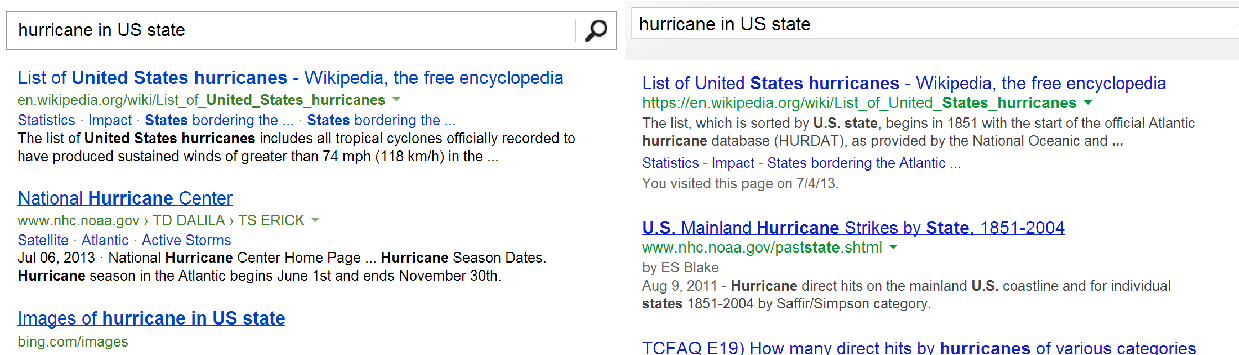
\includegraphics[width=\columnwidth]{images/hurricaneinstates}
  \caption{Search Result of Concept-based Query in Bing and Google}
  \label{fig:exampleGoogle}
\end{figure}

Search engines today return pages {\em about} these abstract concepts, and
that usually means a list of huricanes in the US history for the above
example (see Figure \ref{fig:exampleGoogle}).
It takes the user at least a few
more clicks and scanning through the pages to find the information needed.
Our objectives is to return a list of suggested queries such as:
{\em Katrina in Lousiana},
{\em Sandy in Connecticut},
{\em Dolly in Texas}.

%is trying to do suggestion to concept-based query, which is hard for search engines, because the concepts in query usually contain deep semantic meaning.
%Fig. \ref{fig:exampleGoogle} illustrates the result of Bing and Google towards this kind of query. Specially, \textit{hurricane} and \textit{state} are the concepts. This feature is extremely useful when users cannot come up with specific keywords or they just want to search about abstract concepts.

%\KZ{The figure is not very clear. change to a higher resolution one?
%You can put two eps side by side in one line. Change the query to
%``hurricane in US state'', and re-take the screenshots. Also the way you convert
%to eps is a bit problematic. The size of the image isn't embedded in the eps.
%Use convert in ImageMagick.}

To this end, our main approach utilizes a comprehensive,
probabilistic taxonomy and a search log with access statistics (click-through
rate, etc.). The probabilistic taxonomy, called Probase\cite{wu2012probase},
provides large number of concepts and their instances in is-a relations (e.g.
katrina {\em isa} hurricane) as well as the {\em typicality} of an instance
belonging to a concept. For example, a robin is a {\em typical} bird, but
an ostrich is not. Given a user query, we use this taxonomy to
detect high level concepts in it and translate them into likely instances
to produce a new query, and then return the queries from the query log
which are closest to the newly transformed query.
Next, we present the prototype system in some detail and some preliminary
experimental results.
%
%In order to do the work, we include two utilities -- Probase \cite{wu2012probase} and Stanford Parser \cite{klein2003accurate}. Probase is a large-scale probabilistic taxonomic knowledge base with scores. Its taxonomy can help us recognize concepts and instances and its \textit{typicality} value can tell us how strong the relation is between a concept and an instance. Stanford Parser can help understand the basic semantic structure of users' query.
